%\setchapterimage{fig_00_bis}
\chapter*{Application \arabic{cptApplication} \\ 
 \ifprof Corrigé \else Sujet \fi}

\addcontentsline{toc}{section}{Application \arabic{cptApplication} -- \ifprof Corrigé \else Sujet \fi}

\iflivret \stepcounter{cptApplication} \else
\ifprof  \stepcounter{cptApplication} \else \fi
\fi
\setcounter{question}{0}

%\marginnote{Centrale Supelec TSI 2021.}
%\marginnote{\UPSTIcompetence[2]{C2-03}}
%\begin{marginfigure}
%\centering
%\includegraphics[width=\linewidth]{fig_01}
%\end{marginfigure}



On considère le schéma-blocs suivant. 
\begin{center}
\includegraphics[width=\linewidth]{fig_01}
\end{center}


On a $H_r(p)=K_r \dfrac{1+0,492 p}{1+10,34p+5,1p^2}$ et $K_r = \SI{0,37}{rad.s^{-1}.N^{-1}.m^{-1}}$.
$H_m(p)=\dfrac{0,5}{\left(1+10p \right)\left(1+0,5p \right)}$. Le gain du capteur est de $a=\SI{2}{V.rad^{-1}.s}$.

{On considère que $C(p)=K_P$ et que $C_r(p)=0$.}


\question{Déterminer l'écart statique et l'écart de traînage.}

{On considère que $C(p)=K_P$ et que $C_r(p)$ est une perturbation de type échelon.}

\question{Déterminer l'écart statique et l'écart de traînage.}

{On considère que $C(p)=K_p+\dfrac{1}{T_i p} $ et que $C_r(p)=0$.}

\question{Déterminer l'écart statique et l'écart de traînage.}

On considère que $C(p)=K_p+\dfrac{1}{T_i p} $ et que $C_r(p)$ est une perturbation de type échelon.

\question{Déterminer l'écart statique et l'écart de traînage.}




\ifprof
\begin{center}
\includegraphics[width=\linewidth]{cor_02}
\end{center}

\else
\fi


%\ifprof
%\else
%\noindent\begin{minipage}[c]{.4\linewidth}
%\begin{center}
%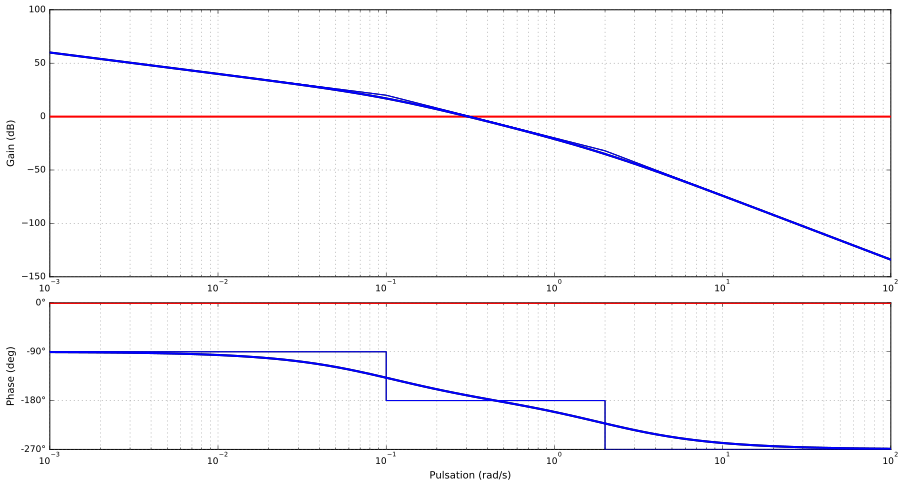
\includegraphics[width=\linewidth]{fig_03}
%\end{center}
%\end{minipage}\hfill
%\begin{minipage}[c]{.46\linewidth}
%\begin{center}
%\includegraphics[width=.9\linewidth]{fig_01}
%\end{center}
%\end{minipage}

\ifprof
\else
\fi

%
%\begin{center}
%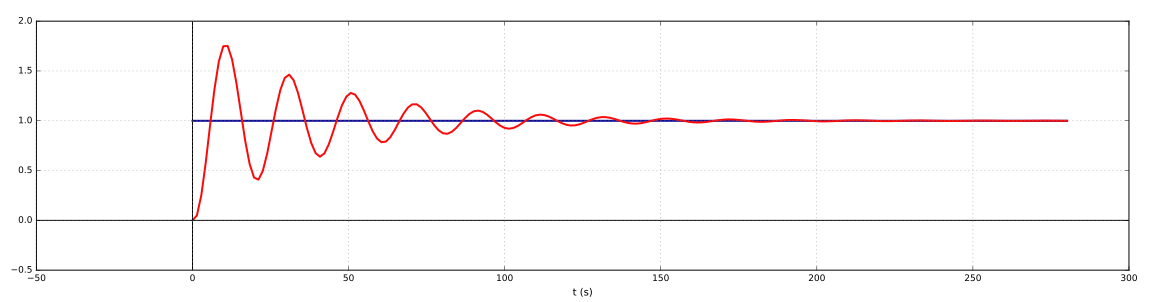
\includegraphics[width=\linewidth]{fig_02}
%\end{center}
%
%\begin{center}
%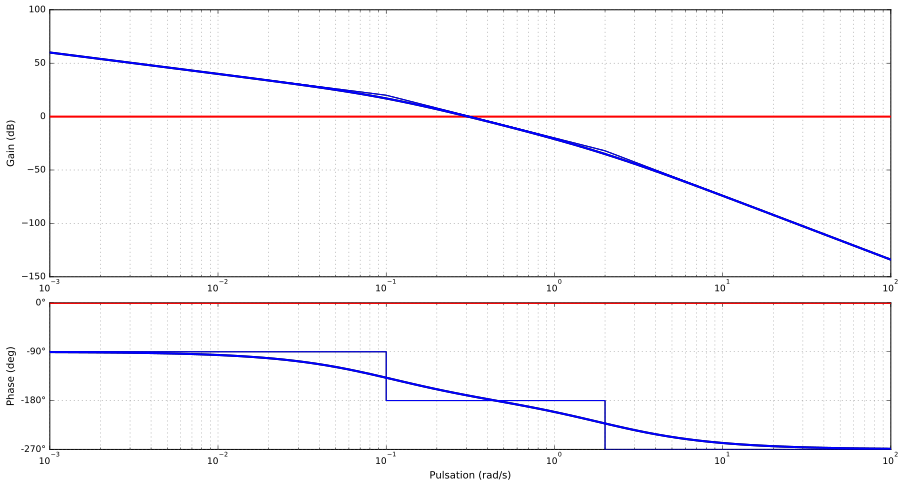
\includegraphics[width=\linewidth]{fig_03}
%\end{center}
%
%\begin{center}
%\includegraphics[width=.8\linewidth]{fig_04}
%\end{center}



%\end{document}
%
%\subsection*{Exercice 3 -- Applications du critère du Revers}
%
%\subparagraph*{}\textit{On donne ci-dessous les lieux de transferts de plusieurs FTBO. Déterminer, à l'aide du critère du Revers si les systèmes sont stables en BF.}
%\subparagraph*{}\textit{Pour les systèmes stables déterminer les marges de gain et de phase.}
%
%\end{multicols}
%
%\begin{center}
%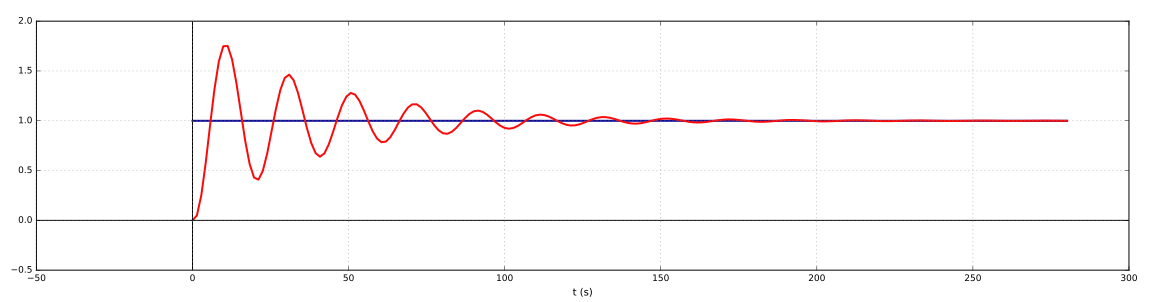
\includegraphics[width=\linewidth]{fig_02}
%\end{center}
%
%\begin{center}
%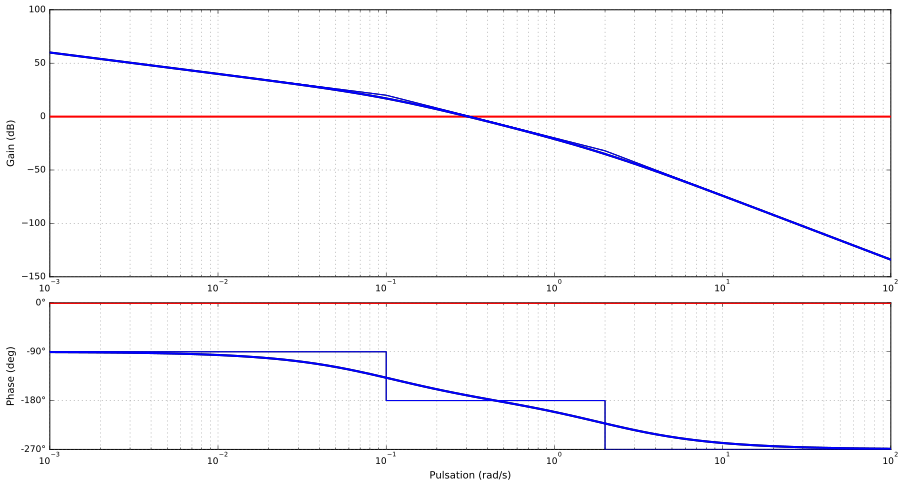
\includegraphics[width=\linewidth]{fig_03}
%\end{center}
%
%\begin{center}
%\includegraphics[width=.8\linewidth]{fig_04}
%\end{center}
%


